\subsection{Lukke}

At ''lukke'' et billede betyder at vi bruger dilation først og dernæst erosion. Med dette vil følgende ske:

\begin{itemize}
	\item Udjævner igen konturene, men
	\item Samler objekter, som ellers kun er forbindet med den tynde forbindelse.
	\item Fjerner ''små'' huller.
	\item Udfylder ''gaps'' i konturen.
\end{itemize}

Ligningen for at lukke et billedet er vist på Figur~\ref{fig:closingeq}.

\begin{figure}[H]
	\centering
	
\includegraphics[width=0.6\linewidth]{figs/spm09/closingeq}
	\caption{Ligning for at ''lukke'' billedet.}
	\label{fig:closingeq}
\end{figure}

Figur~\ref{fig:closing-shape} viser en lukning af et billede. Først hvordan \textit{strel} objektet føres rundt. Så i midten er den færdige lukning tegnet op med fed. I det tredje billede er lukningen farvet op med grå.

\begin{figure}[H]
	\centering
	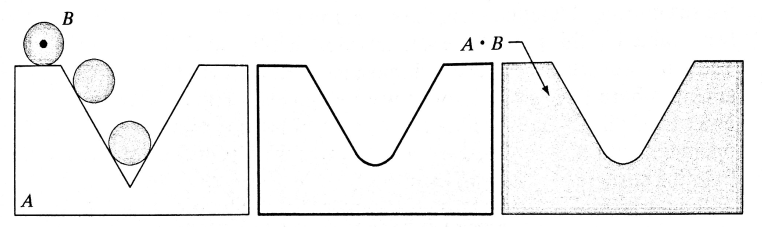
\includegraphics[width=0.9\linewidth]{figs/spm09/closing-shape}
	\caption{Eksempel på hvordan lukning laves.}
	\label{fig:closing-shape}
\end{figure}
